\documentclass[20pt]{article}
\usepackage[left=2cm,right=2cm,top=2cm]{geometry}
\usepackage{physics}
\usepackage{graphicx}

\begin{document}
\title{{\LARGE \textbf{Solving Ising Model for a particular sample}}}
\author{}
\date{}
\maketitle
\section{{\Large Introduction\\}}
The phase transition is a very interesting and also a quite difficult to explain phenomenon in terms of Statistical Mechanics. There are various kind of crystals which shows phase transitions at various temperatures. To explain the behaviour of a metal near critical temperature, to observe the nature of magnetization, energy, specific heat or the magnetic susceptibility of a substance we use some models to explain those theoretically. One of those models is Ising Model. This model was proposed by Ernst Ising initially to explain those behaviours in one dimension. He believed this model fails for higher dimensions. But later Lars Onsager proposed an complicated but very nice solution to the two dimensional Ising Model proving that this model can be useful in more than one dimensions. But proper analytic solution of this in 3D is not yet available. In 3D, this is done by some more approximations like Mean Field Theory or computationally using Monte Carlo Method etc.   \\
\paragraph*{{\large The Ising Model}}
\paragraph*{Hamiltonian\\}

In this Model we consider $N$ sites of a $d$-dimensional lattice where each lattice site consists of spins(i.e. magnetic moments). Physical phenomenons like magnetic moments, susceptibility, specific heat etc. are explained in this model by considering the interactions between the spins. The simplest case is considering only the nearest  neighbour interactions. The Hamiltonian of the system depends on the interactions of the spins and an exchange integral term($J$) which has the dimension of energy. If we write the eigenvalue of the $i^{th}$ spin as $s_i$, then the Hamiltonian will be,\\


$H(s_1,s_2,...s_N)=-J \sum_{nearest.neighbour} s_i s_j$ \\


If $J>0$ the neighbouring spins prefer to be aligned (i.e. $ \uparrow \uparrow$ or $ \downarrow \downarrow$). Such a spin system is called ferromagnet. And for $J<0$, neighbouring spins are anti-aligned($\uparrow \downarrow$), these are called anti-ferromagnet.  \\
In presence of an external magnetic field $B$, this Hamiltonian takes the form:\\

$H(s_1,s_2,...s_N)=-J \sum_{nearest.neighbour} s_i s_j - B \sum_{i} s_i$

\paragraph{Periodic Boundary Condition \\}
To solve this model we use an assumption called periodic boundary condition. This assumes, say in one dimension, the $(N+1)^{th}$ spin is the $1^{st}$ spin again. Which makes the whole oneD lattice like a ring. And in twoD this assumption makes the  lattice sheet a torus. This assumptions makes the model easier to solve in both oneD and twoD. But in three dimensional case we can use another assumption called \textit{The Mean Field Approximation } to solve the system.\\

\paragraph{ Mean Field Approximation\\}
In the mean field approximation, the basic assumption is that instead of interacting directly with the neighbouring spins, each spin interact with each other with a 'mean field' which follows from the mean orientation of the neighbouring spins.\\

Here for the term in the Hamiltonian $s_i s_j$, we write\\

$s_i s_j = [(s_i - m)+m][(s_j - m)+ m]$,\\ 

here $m$ is the mean field that the spins interact with. Thus,\\


$s_i s_j  = (s_i - m)(s_j - m) + m(s_j - m) + m(s_i - m)+ m^2$ \\


Here we identify, $(s_i - m)$ and $(s_j - m)$ are the fluctuations of the individual spins from the mean field. Though these fluctuations for individual spins may not be small but the product fluctuations of two different neighbouring spins  may be neglected while doing the sum $\sum_{n.n}$.\\
Thus, the Hamiltonian becomes:\\

$H_{m.f} = -J \sum_{n.n} [m (s_i - m) + m (s_j - m)] - B \sum_{i} s_i$\\

$\implies H_{m.f} = \frac{1}{2} J N q m^2 - (J q m + B)\sum_{i} s_i $ \\

Here $N$ is the total number of lattice sites and $q$ is the number of nearest neighbours. The $\frac{1}{2}$ comes because we do the sum over pairs not on the individual sites.\\
Thus if we see the new mean field Hamiltonian carefully, we see that it has removed the interactions and an effective magnetic filed is in action:\\

$B_{eff} = B + J q m$\\. 

From here, in \textit{Canonical Ensemble}, we can write a partition function,\\

$Z= \sum_{s_i} \exp[-\beta H(s_i)]$\\
 
and the average magnetization:\\
 
$m= \frac{1}{N} \sum_{i} s_i = \frac{1}{N \beta} \pdv {log(Z)}{\beta}$\\
  

This is the core concept of the mean field theory. Here we will try to solve the Hamiltonian i.e. try to write the partition function for a specific kind of lattice, and calculate some properties like magnetization, specific heat etc.\\
Let's know about the sample first.\\

\section*{The Sample}
\paragraph{ Crystal Structure\\}
The sample we are working with is generally denoted by $RNiO_3$ perovskites. Here $R$ is rare earth elements.This kind of materials has a structure of orthorhombically distorted perovskites. The ideal cubic structure of $R$ and $Ni$ has a 3D array of  corner sharing $Ni O_6$ octahedra.

\begin{figure}[h!]
\centering
	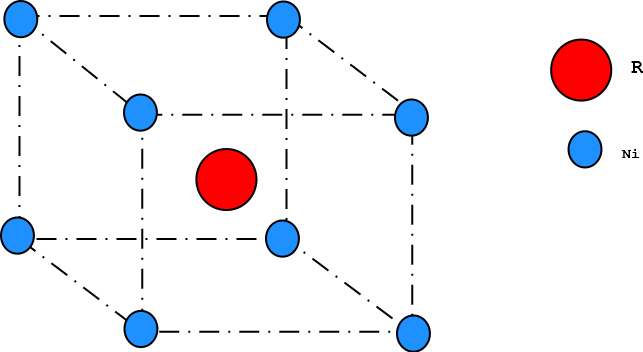
\includegraphics[width=0.4\textwidth]{RNiO3_2.png}
	\caption{The basic Cubic Structure without the Oxygen}
	\end{figure}
	
Figure 1 shows the basic ideal cubic structure where at the centre there is an $R$ and all the corners have $Ni$ in it.
\begin{figure}[h!]
\centering
	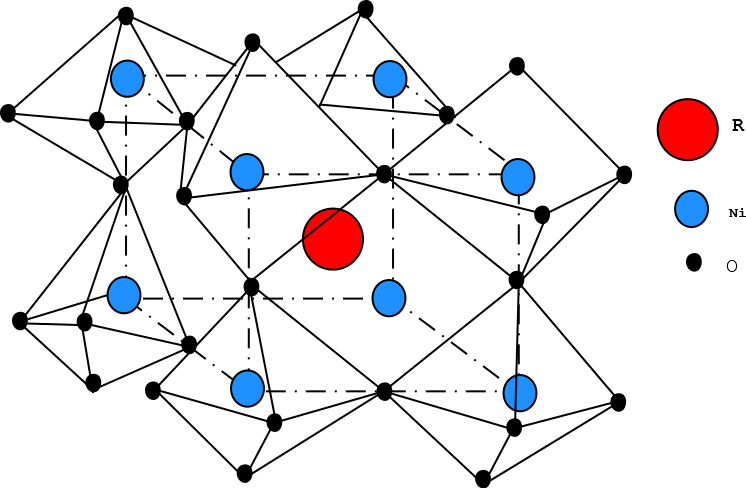
\includegraphics[width=0.4\textwidth]{RNiO3.png}
	\caption{The Ideal Perovskite Structure }
	\end{figure}

The $Ni$-s at the corners have 6 $O$-s around it (Figure 2). This makes it a $NiO_6$ structure, but Oxygens are shared by the Nickels resulting the whole structure to be $RNiO_3$.\\

\paragraph*{Spin Structure\\}
Generally while solving the Ising Model we take the spins of the lattice points as $\pm1$ , but in case of real crystals like this we can have a mixed spin structures. Here we will take spins of $LaNiO_3$ which belongs to the class of $RNiO_3$.\\
We know that the term symbols for $Ni$, $O$ and $La$ are $^3F_4$, $^3P_2$ and  $^2D_{\frac{3}{2}}$ respectively. Thus their spins are $\pm 1$, $\pm 1$ and $\pm\frac{1}{2}$ respectively. 






\end{document}
